% Options for packages loaded elsewhere
\PassOptionsToPackage{unicode}{hyperref}
\PassOptionsToPackage{hyphens}{url}
%
\documentclass[
]{book}
\usepackage{lmodern}
\usepackage{amsmath}
\usepackage{ifxetex,ifluatex}
\ifnum 0\ifxetex 1\fi\ifluatex 1\fi=0 % if pdftex
  \usepackage[T1]{fontenc}
  \usepackage[utf8]{inputenc}
  \usepackage{textcomp} % provide euro and other symbols
  \usepackage{amssymb}
\else % if luatex or xetex
  \usepackage{unicode-math}
  \defaultfontfeatures{Scale=MatchLowercase}
  \defaultfontfeatures[\rmfamily]{Ligatures=TeX,Scale=1}
\fi
% Use upquote if available, for straight quotes in verbatim environments
\IfFileExists{upquote.sty}{\usepackage{upquote}}{}
\IfFileExists{microtype.sty}{% use microtype if available
  \usepackage[]{microtype}
  \UseMicrotypeSet[protrusion]{basicmath} % disable protrusion for tt fonts
}{}
\makeatletter
\@ifundefined{KOMAClassName}{% if non-KOMA class
  \IfFileExists{parskip.sty}{%
    \usepackage{parskip}
  }{% else
    \setlength{\parindent}{0pt}
    \setlength{\parskip}{6pt plus 2pt minus 1pt}}
}{% if KOMA class
  \KOMAoptions{parskip=half}}
\makeatother
\usepackage{xcolor}
\IfFileExists{xurl.sty}{\usepackage{xurl}}{} % add URL line breaks if available
\IfFileExists{bookmark.sty}{\usepackage{bookmark}}{\usepackage{hyperref}}
\hypersetup{
  pdftitle={Lectures on Quantum Information Science},
  pdfauthor={Artur Ekert},
  hidelinks,
  pdfcreator={LaTeX via pandoc}}
\urlstyle{same} % disable monospaced font for URLs
\usepackage{longtable,booktabs}
\usepackage{calc} % for calculating minipage widths
% Correct order of tables after \paragraph or \subparagraph
\usepackage{etoolbox}
\makeatletter
\patchcmd\longtable{\par}{\if@noskipsec\mbox{}\fi\par}{}{}
\makeatother
% Allow footnotes in longtable head/foot
\IfFileExists{footnotehyper.sty}{\usepackage{footnotehyper}}{\usepackage{footnote}}
\makesavenoteenv{longtable}
\usepackage{graphicx}
\makeatletter
\def\maxwidth{\ifdim\Gin@nat@width>\linewidth\linewidth\else\Gin@nat@width\fi}
\def\maxheight{\ifdim\Gin@nat@height>\textheight\textheight\else\Gin@nat@height\fi}
\makeatother
% Scale images if necessary, so that they will not overflow the page
% margins by default, and it is still possible to overwrite the defaults
% using explicit options in \includegraphics[width, height, ...]{}
\setkeys{Gin}{width=\maxwidth,height=\maxheight,keepaspectratio}
% Set default figure placement to htbp
\makeatletter
\def\fps@figure{htbp}
\makeatother
\setlength{\emergencystretch}{3em} % prevent overfull lines
\providecommand{\tightlist}{%
  \setlength{\itemsep}{0pt}\setlength{\parskip}{0pt}}
\setcounter{secnumdepth}{5}
\usepackage{booktabs}
\ifluatex
  \usepackage{selnolig}  % disable illegal ligatures
\fi
\usepackage[]{natbib}
\bibliographystyle{apalike}

\title{Lectures on Quantum Information Science}
\author{Artur Ekert}
\date{2020-11-14}

\usepackage{amsthm}
\newtheorem{theorem}{Theorem}[chapter]
\newtheorem{lemma}{Lemma}[chapter]
\newtheorem{corollary}{Corollary}[chapter]
\newtheorem{proposition}{Proposition}[chapter]
\newtheorem{conjecture}{Conjecture}[chapter]
\theoremstyle{definition}
\newtheorem{definition}{Definition}[chapter]
\theoremstyle{definition}
\newtheorem{example}{Example}[chapter]
\theoremstyle{definition}
\newtheorem{exercise}{Exercise}[chapter]
\theoremstyle{remark}
\newtheorem*{remark}{Remark}
\newtheorem*{solution}{Solution}
\begin{document}
\maketitle

{
\setcounter{tocdepth}{1}
\tableofcontents
}
\hypertarget{overview}{%
\chapter*{Overview}\label{overview}}
\addcontentsline{toc}{chapter}{Overview}

\hypertarget{quantum-interference}{%
\chapter{Quantum interference}\label{quantum-interference}}

\begin{quote}
About complex numbers, called probability amplitudes, that, unlike probabilities, can cancel each other out, leading to quantum interference and qualitatively new ways of processing information.
\end{quote}

The classical theory of computation does not usually refer to physics.
Pioneers such as Alan Turing, Alonzo Church, Emil Post and Kurt Gödel managed to capture the correct classical theory by intuition alone and, as a result, it is often falsely assumed that its foundations are self-evident and purely abstract.
They are not!\footnote{Computation is a physical process. Computation is a physical process. Computation is \ldots{}}

The concepts of information and computation can be properly formulated only in the context of a physical theory --- information is stored, transmitted and processed always by \emph{physical} means.
Computers are physical objects and computation is a physical process.
Indeed, any computation, classical or quantum, can be viewed in terms of physical experiments, which produce \textbf{outputs} that depend on initial preparations called \textbf{inputs}.
Once we abandon the classical view of computation as a purely logical notion independent of the laws of physics it becomes clear that whenever we improve our knowledge about physical reality, we may also gain new means of computation.
Thus, from this perspective, it is not very surprising that the discovery of quantum mechanics in particular has changed our understanding of the nature of computation.
In order to explain what makes quantum computers so different from their classical counterparts, we begin with the rudiments of quantum theory.

\hypertarget{two-basic-rules}{%
\section{Two basic rules}\label{two-basic-rules}}

Quantum theory, at least at some instrumental level, can be viewed as a modification of probability theory.
We replace positive numbers (probabilities) with complex numbers \(z\) (called \textbf{probability amplitudes}) such that the squares of their absolute values, \(|z|^2\), are interpreted as probabilities.

\begin{definition}
\protect\hypertarget{def:unlabeled-div-1}{}\label{def:unlabeled-div-1}

The correspondence between probability amplitude \(z\) and probability \(p=|z|^2\) is known as \textbf{Born's Rule}.

\end{definition}

The rules for combining amplitudes are very reminiscent of the rules for combining probabilities:

\begin{enumerate}
\def\labelenumi{\arabic{enumi}.}
\tightlist
\item
  Whenever something can happen in a sequence of independent steps, we multiply the amplitudes of each step.
\end{enumerate}

\begin{center}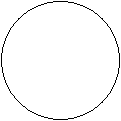
\includegraphics{quantum-site_files/figure-latex/unnamed-chunk-1-1} \end{center}

\begin{enumerate}
\def\labelenumi{\arabic{enumi}.}
\setcounter{enumi}{1}
\tightlist
\item
  Whenever something can happen in several alternative ways, we add the amplitudes for each separate way.
\end{enumerate}

That's it!
These two rules are basically all you need to manipulate amplitudes in any physical process, no matter how complicated.\footnote{We will, however, amend the two rules later on when we touch upon particle statistics.}
They are universal and apply to any physical system, from elementary particles through atoms and molecules to white dwarfs stars.
They also apply to information, since, as we have already emphasised, information is physical.
The two rules look deceptively simple but, as you will see in a moment, their consequences are anything but trivial.

\hypertarget{quantum-interference-the-failure-of-probability-theory}{%
\section{Quantum interference (the failure of probability theory)}\label{quantum-interference-the-failure-of-probability-theory}}

\hypertarget{superpositions}{%
\section{Superpositions}\label{superpositions}}

\hypertarget{interferometers}{%
\section{Interferometers}\label{interferometers}}

\hypertarget{qubits-gates-and-circuits}{%
\section{Qubits, gates, and circuits}\label{qubits-gates-and-circuits}}

\hypertarget{quantum-decoherence}{%
\section{Quantum decoherence}\label{quantum-decoherence}}

\hypertarget{computation-deterministic-probabilistic-and-quantum}{%
\section{Computation: deterministic, probabilistic, and quantum}\label{computation-deterministic-probabilistic-and-quantum}}

\hypertarget{computational-complexity}{%
\section{Computational complexity}\label{computational-complexity}}

\hypertarget{outlook}{%
\section{Outlook}\label{outlook}}

\hypertarget{notes-and-exercises}{%
\section{Notes and Exercises}\label{notes-and-exercises}}

\hypertarget{supplement-physics-against-logic-via-beamsplitters}{%
\section{Supplement: Physics against logic, via beamsplitters}\label{supplement-physics-against-logic-via-beamsplitters}}

\hypertarget{supplement-quantum-interference-revisited-still-about-beamsplitters}{%
\section{Supplement: Quantum interference revisited (still about beamsplitters)}\label{supplement-quantum-interference-revisited-still-about-beamsplitters}}

\hypertarget{qubits}{%
\chapter{Qubits}\label{qubits}}

\hypertarget{measurements}{%
\chapter{Measurements}\label{measurements}}

\hypertarget{quantum-entanglement}{%
\chapter{Quantum entanglement}\label{quantum-entanglement}}

\hypertarget{quantum-algorithms}{%
\chapter{Quantum algorithms}\label{quantum-algorithms}}

\hypertarget{bells-theorem}{%
\chapter{Bell's theorem}\label{bells-theorem}}

\hypertarget{decoherence-and-elements-of-quantum-error-correction}{%
\chapter{Decoherence, and elements of quantum error correction}\label{decoherence-and-elements-of-quantum-error-correction}}

\hypertarget{density-matrices}{%
\chapter{Density matrices}\label{density-matrices}}

\hypertarget{quantum-channels-or-cp-maps}{%
\chapter{Quantum channels (or CP maps)}\label{quantum-channels-or-cp-maps}}

\hypertarget{quantum-error-correction-and-fault-tolerance}{%
\chapter{Quantum error correction and fault tolerance}\label{quantum-error-correction-and-fault-tolerance}}

  \bibliography{book.bib}

\end{document}
